

% Compact single-column paper/memo format.

\documentclass[10pt,a4paper,parskip=half-]{scrartcl}
\usepackage[margin=1.6cm]{geometry}
\usepackage[T1]{fontenc}
\usepackage[utf8]{inputenc}
\usepackage{lmodern}
\usepackage{amsmath}
\usepackage{amsfonts}
\usepackage{amssymb}
\usepackage{graphicx}
\usepackage{float}
\usepackage{placeins}
\usepackage{booktabs}
\usepackage{array}
\usepackage{adjustbox}
\usepackage{url}
\usepackage{xcolor}
\usepackage{tikz}
\usepackage[nocompress]{cite}
\usepackage{pdflscape}
\usepackage{microtype}
\usetikzlibrary{positioning,arrows.meta,shapes.geometric,fit,backgrounds,calc}
% --- Workflow-overview figure palette (mirrors the Mermaid version in doc/workflow_overview.md) ---
\definecolor{wfIndigo}{HTML}{312E81}
\definecolor{wfIndigoLight}{HTML}{E0E7FF}
\definecolor{wfIndigoMid}{HTML}{4F46E5}
\definecolor{wfAmberDark}{HTML}{D97706}
\definecolor{wfAmberLight}{HTML}{FEF3C7}
\definecolor{wfAmberText}{HTML}{78350F}
\definecolor{wfEmeraldDark}{HTML}{059669}
\definecolor{wfEmeraldLight}{HTML}{D1FAE5}
\definecolor{wfEmeraldText}{HTML}{064E3B}
\definecolor{wfEmeraldBg}{HTML}{ECFDF5}
\definecolor{wfPinkDark}{HTML}{DB2777}
\definecolor{wfPinkLight}{HTML}{FCE7F3}
\definecolor{wfPinkText}{HTML}{831843}
\definecolor{wfBlueDark}{HTML}{2563EB}
\definecolor{wfBlueLight}{HTML}{DBEAFE}
\definecolor{wfBlueText}{HTML}{1E3A8A}
\definecolor{wfBlueBg}{HTML}{EFF6FF}
\definecolor{wfViolet}{HTML}{7C3AED}
\definecolor{wfVioletDark}{HTML}{5B21B6}
\definecolor{wfRoseDark}{HTML}{E11D48}
\definecolor{wfRoseLight}{HTML}{FFE4E6}
\definecolor{wfRoseText}{HTML}{881337}
\definecolor{wfRoseBg}{HTML}{FFF1F2}
\definecolor{wfSlate}{HTML}{475569}
\newcolumntype{L}[1]{>{\raggedright\arraybackslash}p{#1}}

\newcommand{\widecomparisonplot}[1]{\includegraphics[width=0.76\textwidth]{#1}}

\newcommand{\encodingexampleplot}[1]{\includegraphics[width=0.42\linewidth]{#1}}
\newcommand{\subfigtext}[1]{\par\smallskip{\footnotesize #1\par}}
\setlength{\textfloatsep}{8pt plus 2pt minus 2pt}
\setlength{\floatsep}{8pt plus 2pt minus 2pt}
\setlength{\intextsep}{8pt plus 2pt minus 2pt}
\raggedbottom
\hyphenation{op-tical net-works semi-conduc-tor}


\begin{document}
\title{Controlled Inversion of Image-Based Time-Series Encodings: Operational Decoders for GAF, RP, and MTF Representations}
\author{Adriano~García-Giralda~Milena\thanks{Research collaborator with the MYDASS Research Group, University of Granada.}
\and Francisco~García~Moreno\thanks{Department of Computer Languages and Systems, University of Granada.}
\and José Antonio Jiménez Madrid\thanks{Department of Algebra, University of Granada.}
\and
María Bermúdez Edo\thanks{Department of Computer Languages and Systems, University of Granada.}
}
\date{2026}







\maketitle
\begin{abstract}
Image-based time-series encodings expose temporal structure to image-domain models, but their usefulness for signal generation depends on whether the encoded image can be mapped back to the time domain. We study this controlled inverse problem for Recurrence Plots (RP), Gramian Angular Summation and Difference Fields (GASF/GADF), and Markov Transition Fields (MTF). We propose three operational decoders: a signed-RP decoder based on two-dimensional classical multidimensional scaling, adjacent-state overlap, and signed orientation selection; a closed-form, restricted-branch GADF decoder with image-derived boundary anchoring and multi-pivot averaging; and a spectral MTF decoder that orders recovered quantile states through a Fiedler vector. A GASF diagonal inverse is retained as a prior-art baseline.

On 8,172 triaxial WISDM windows, evaluated with pointwise error, polynomial trend similarity, and six original-trained classifiers under window-level and grouped subject-out three-fold protocols, RP, GASF, and GADF form a near-original tier. Their global MAEs are 0.0148, 0.0205, and 0.0157\,m/s$^2$, with Pearson correlation approximately one; subject-level equivalence tests also place their classification accuracy within two percentage points of the raw signal. MTF is the only many-to-one reconstruction and is consistently less faithful. These results concern images produced by known encoders with known settings; they establish controlled reconstruction, not generative augmentation.
\end{abstract}

\noindent\textbf{Keywords:}
Markov Transition Fields, Recurrence Plots, Gramian Angular Fields, Gramian Angular Difference Field, Time Series Reconstruction, Image Encoding, Accelerometer Data, Machine Learning.
\par\bigskip




\section{Introduction}
\label{sec:introduction}
Time-series images such as Recurrence Plots (RP), Markov Transition Fields (MTF), and Gramian Angular Fields (GAF) allow image-domain models to operate on temporal relations rather than directly on raw samples \cite{wang2015encoding,wang2015encoding2}. For triaxial accelerometer windows, each axis is encoded separately and stored as one image channel. This representation is attractive for image generation, but it raises a prerequisite question: does an encoded image retain enough information to recover the underlying signal?

We address that inverse problem under controlled conditions. Every evaluated image is the deterministic output of a known encoder; encoder settings are known, and per-window amplitude calibration is used only when reconstruction in physical units is requested. We do not train a diffusion model or a GAN, and we make no claim that an arbitrary generated image is automatically physically valid. Instead, we establish which representations can return faithfully to the time domain before generative augmentation is attempted.

The study compares four encodings under one protocol: visual inspection, pointwise error, cubic-trend similarity, and robustness of six classifiers trained on the original signals. Both stratified window-level and grouped subject-out three-fold splits are reported on the WISDM smartwatch accelerometer data. Figure~\ref{fig:workflow_overview} summarises the workflow.

The main contributions are:

\begin{itemize}
    \item a signed-RP decoder for continuous Lu--Tong recurrence plots of overlapping states, combining two-dimensional classical multidimensional scaling, consecutive-state overlap alignment, and signed orientation selection;

    \item a closed-form GADF decoder whose restricted angular branch, image-derived boundary anchor, and multi-pivot reconstruction make the normalised inverse operational without per-window amplitude metadata;
    \item a Fiedler-vector MTF decoder that recovers a representative quantile trajectory, with GASF diagonal inversion retained as a controlled prior-art baseline; and
    \item a unified evaluation showing that RP, GASF, and GADF reconstruct at the 8-bit quantisation floor and preserve original-trained classification, whereas MTF remains a lossy, classifier-oriented representation.
\end{itemize}

\begin{figure}[!htbp]
\centering
\resizebox{\textwidth}{!}{%
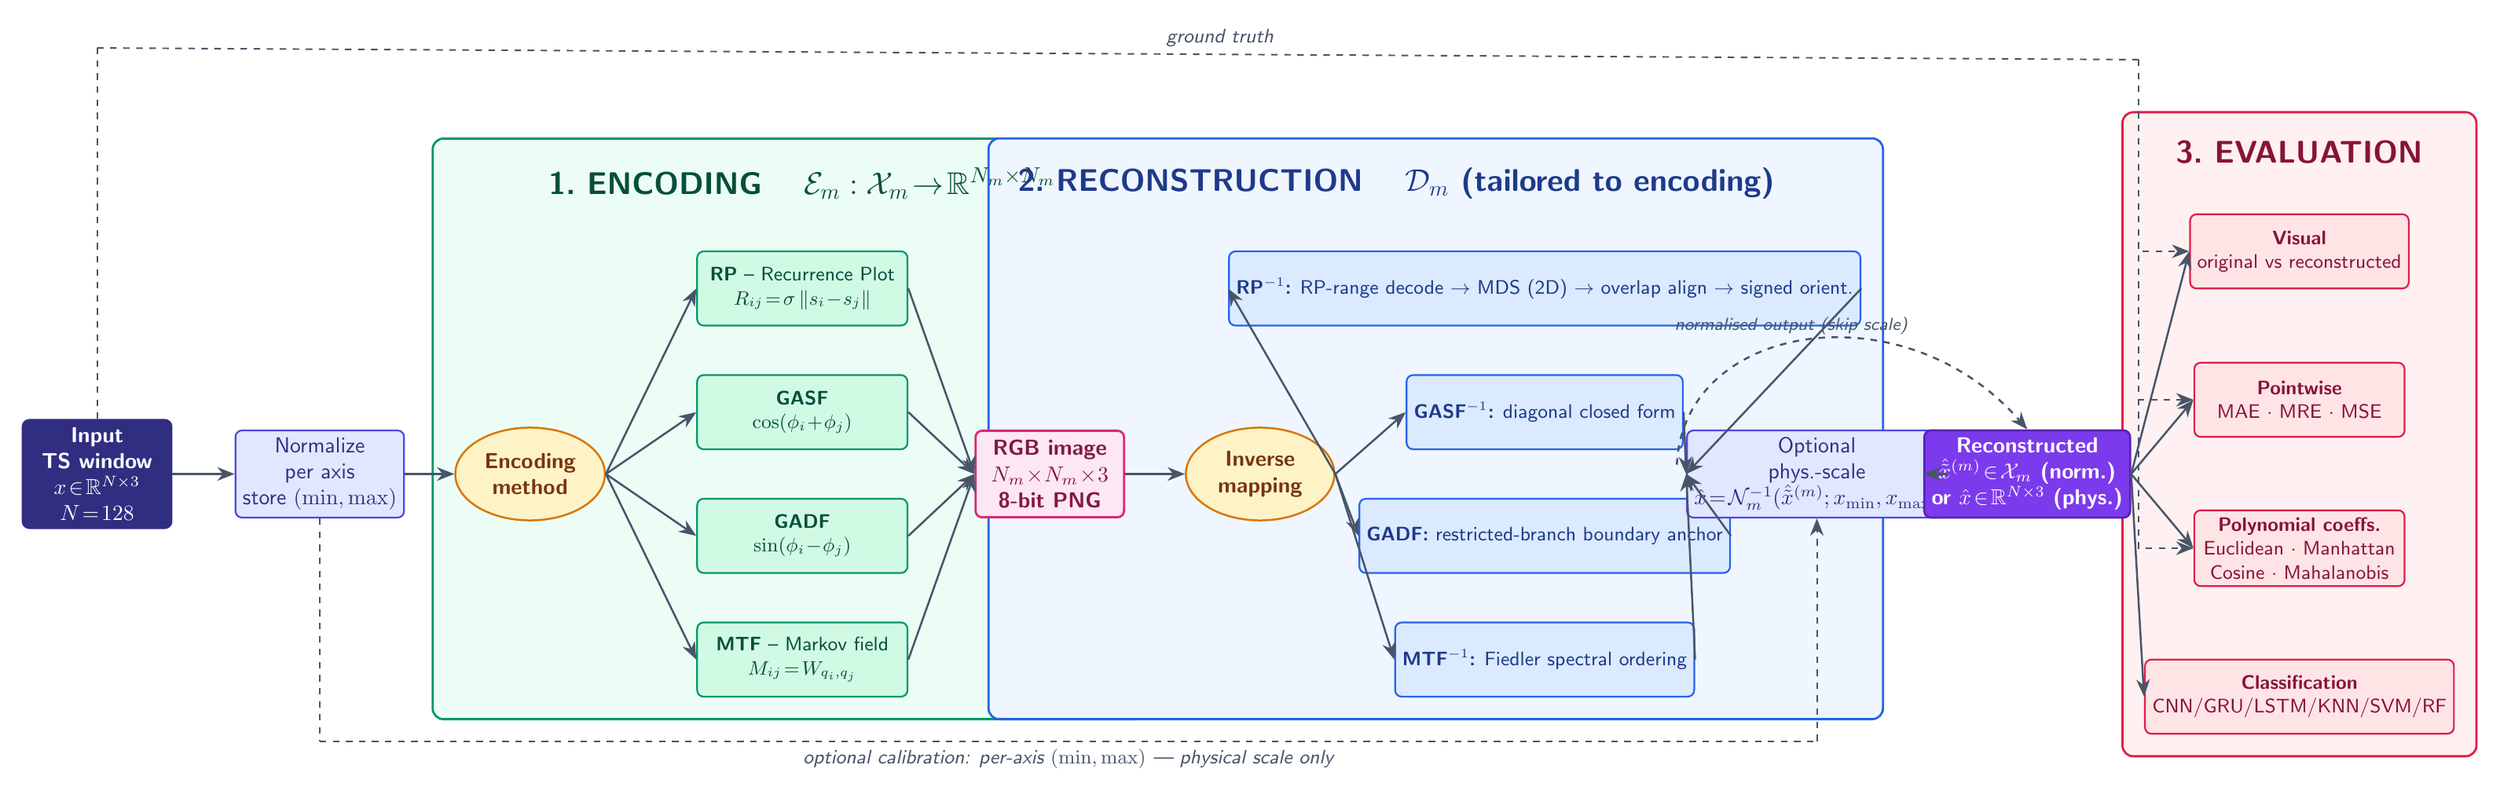
\begin{tikzpicture}[
  font=\sffamily,
  >={Stealth[length=2.8mm,width=2.2mm]},
  input/.style ={rectangle, rounded corners=3pt, draw=wfIndigo, line width=1pt,
                 fill=wfIndigo, text=white, align=center,
                 minimum height=14mm, minimum width=24mm, font=\sffamily\bfseries},
  pre/.style   ={rectangle, rounded corners=3pt, draw=wfIndigoMid, line width=0.8pt,
                 fill=wfIndigoLight, text=wfIndigo, align=center,
                 minimum height=14mm, minimum width=24mm, font=\sffamily},
  router/.style={ellipse, draw=wfAmberDark, line width=0.9pt,
                 fill=wfAmberLight, text=wfAmberText, align=center,
                 minimum width=24mm, minimum height=15mm,
                 font=\sffamily\bfseries},
  enc/.style   ={rectangle, rounded corners=3pt, draw=wfEmeraldDark, line width=0.8pt,
                 fill=wfEmeraldLight, text=wfEmeraldText, align=center,
                 minimum height=12mm, minimum width=34mm, font=\sffamily\small},
  img/.style   ={rectangle, rounded corners=3pt, draw=wfPinkDark, line width=1pt,
                 fill=wfPinkLight, text=wfPinkText, align=center,
                 minimum height=14mm, minimum width=24mm, font=\sffamily\bfseries},
  rec/.style   ={rectangle, rounded corners=3pt, draw=wfBlueDark, line width=0.8pt,
                 fill=wfBlueLight, text=wfBlueText, align=center,
                 minimum height=12mm, minimum width=40mm, font=\sffamily\small},
  outputnode/.style={rectangle, rounded corners=3pt, draw=wfVioletDark, line width=1pt,
                 fill=wfViolet, text=white, align=center,
                 minimum height=14mm, minimum width=24mm, font=\sffamily\bfseries},
  eval/.style  ={rectangle, rounded corners=3pt, draw=wfRoseDark, line width=0.8pt,
                 fill=wfRoseLight, text=wfRoseText, align=center,
                 minimum height=12mm, minimum width=34mm, font=\sffamily\small},
  arrow/.style ={->, draw=wfSlate, line width=0.9pt},
  gt/.style    ={->, draw=wfSlate, dashed, line width=0.7pt},
]
  % ============ MAIN HORIZONTAL FLOW ============
  \node[input]  (A) at ( 0.0, 0)   {Input\\TS window\\$x\!\in\!\mathbb{R}^{N\times 3}$\\$N\!=\!128$};
  \node[pre]    (B) at ( 3.6, 0)   {Normalize\\per axis\\store $(\min,\max)$};
  \node[router] (C) at ( 7.0, 0)   {Encoding\\method};
  \node[enc] (RP)   at (11.4, 3.0) {\textbf{RP} -- Recurrence Plot\\$R_{ij}\!=\!\sigma\,\lVert s_i\!-\!s_j\rVert$};
  \node[enc] (GASF) at (11.4, 1.0) {\textbf{GASF}\\$\cos(\phi_i\!+\!\phi_j)$};
  \node[enc] (GADF) at (11.4,-1.0) {\textbf{GADF}\\$\sin(\phi_i\!-\!\phi_j)$};
  \node[enc] (MTF)  at (11.4,-3.0) {\textbf{MTF} -- Markov field\\$M_{ij}\!=\!W_{q_i,q_j}$};

  \node[img]    (IMG) at (15.4, 0) {RGB image\\$N_m\!\times\!N_m\!\times\!3$\\8-bit PNG};
  \node[router] (D)   at (18.8, 0) {Inverse\\mapping};
  \node[rec] (R1) at (23.4, 3.0) {\textbf{RP$^{-1}$:} RP-range decode $\to$ MDS (2D) $\to$ overlap align $\to$ signed orient.};

  \node[rec] (R2) at (23.4, 1.0) {\textbf{GASF$^{-1}$:} diagonal closed form};
  \node[rec] (R3) at (23.4,-1.0) {\textbf{GADF:} restricted-branch boundary anchor};
  \node[rec] (R4) at (23.4,-3.0) {\textbf{MTF$^{-1}$:} Fiedler spectral ordering};
  \node[pre]  (E) at (27.8, 0) {Optional\\phys.-scale\\$\hat{x}\!=\!\mathcal{N}_m^{-1}(\hat{\tilde{x}}^{(m)};x_{\min},x_{\max})$};
  \node[outputnode] (F) at (31.2, 0) {Reconstructed\\$\hat{\tilde{x}}^{(m)}\!\in\!\mathcal{X}_m$ (norm.)\\or $\hat{x}\!\in\!\mathbb{R}^{N\times 3}$ (phys.)};
  \node[eval] (V1) at (35.6, 3.6) {\textbf{Visual}\\original vs reconstructed};
  \node[eval] (V2) at (35.6, 1.2) {\textbf{Pointwise}\\MAE $\cdot$ MRE $\cdot$ MSE};
  \node[eval] (V3) at (35.6,-1.2) {\textbf{Polynomial coeffs.}\\Euclidean $\cdot$ Manhattan\\Cosine $\cdot$ Mahalanobis};
  \node[eval] (V4) at (35.6,-3.6) {\textbf{Classification}\\CNN/GRU/LSTM/KNN/SVM/RF};

  % ============ SUBGRAPH TITLES (live inside the backgrounds) ============
  \node[font=\sffamily\Large\bfseries, text=wfEmeraldText]
        (encTitle) at (11.4, 4.7) {1.\ ENCODING \;\; $\mathcal{E}_m:\mathcal{X}_m\!\to\!\mathbb{R}^{N_m\times N_m}$};
  \node[font=\sffamily\Large\bfseries, text=wfBlueText]
        (recTitle) at (21.0, 4.7) {2.\ RECONSTRUCTION \;\; $\mathcal{D}_m$ (tailored to encoding)};
  \node[font=\sffamily\Large\bfseries, text=wfRoseText]
        (evalTitle) at (35.6, 5.2) {3.\ EVALUATION};

  % ============ SOLID ARROWS (signal / image path) ============
  \draw[arrow] (A.east) -- (B.west);
  \draw[arrow] (B.east) -- (C.west);
  \draw[arrow] (C.east) -- (RP.west);
  \draw[arrow] (C.east) -- (GASF.west);
  \draw[arrow] (C.east) -- (GADF.west);
  \draw[arrow] (C.east) -- (MTF.west);
  \draw[arrow] (RP.east)   -- (IMG.west);
  \draw[arrow] (GASF.east) -- (IMG.west);
  \draw[arrow] (GADF.east) -- (IMG.west);
  \draw[arrow] (MTF.east)  -- (IMG.west);
  \draw[arrow] (IMG.east) -- (D.west);
  \draw[arrow] (D.east) -- (R1.west);
  \draw[arrow] (D.east) -- (R2.west);
  \draw[arrow] (D.east) -- (R3.west);
  \draw[arrow] (D.east) -- (R4.west);
  \draw[arrow] (R1.east) -- (E.west);
  \draw[arrow] (R2.east) -- (E.west);
  \draw[arrow] (R3.east) -- (E.west);
  \draw[arrow] (R4.east) -- (E.west);
  \draw[arrow] (E.east) -- (F.west);
  % optional bifurcation: decoder output consumed directly in the normalised domain, bypassing the physical-scale node E
  \draw[arrow, dashed] ($(E.west)+(-0.15,0.15)$) .. controls +(0.1,2.3) and +(-2.0,2.3) .. (F.north)
        node[pos=0.46, above, font=\sffamily\footnotesize\itshape, text=wfSlate] {normalised output (skip scale)};
  \draw[arrow] (F.east) -- (V1.west);
  \draw[arrow] (F.east) -- (V2.west);
  \draw[arrow] (F.east) -- (V3.west);
  \draw[arrow] (F.east) -- (V4.west);


  % ============ DASHED ARROWS (side information) ============
  % --- ground-truth window routed above the subgraphs ---
  \coordinate (gtUp)    at ($(A.north) + (0,6.0)$);

  \coordinate (gtPivot) at (33.0, 6.7);
  \draw[gt, -] (A.north) -- (gtUp);
  \draw[gt, -] (gtUp) -- (gtPivot)
        node[pos=0.55, above, font=\sffamily\small\itshape, text=wfSlate] {ground truth};
  \draw[gt] (gtPivot) |- (V1.west);
  \draw[gt] (gtPivot) |- (V2.west);
  \draw[gt] (gtPivot) |- (V3.west);
  % --- (min, max) metadata routed below the subgraphs ---
  \coordinate (mdL) at ($(B.south) + (0,-3.6)$);
  \coordinate (mdR) at ($(E.south) + (0,-3.6)$);
  \draw[gt, -] (B.south) -- (mdL);
  \draw[gt, -] (mdL) -- (mdR)
        node[midway, below, font=\sffamily\small\itshape, text=wfSlate]
        {optional calibration: per-axis $(\min,\max)$ --- physical scale only};
  \draw[gt] (mdR) -- (E.south);

  % ============ SUBGRAPH BACKGROUNDS ============
  \begin{scope}[on background layer]
    \node[fit=(C)(RP)(MTF)(IMG)(encTitle),
          draw=wfEmeraldDark, line width=1pt, fill=wfEmeraldBg,
          rounded corners=5pt, inner sep=3.5mm] {};
    \node[fit=(D)(R1)(R4)(recTitle),
          draw=wfBlueDark, line width=1pt, fill=wfBlueBg,
          rounded corners=5pt, inner sep=3.5mm] {};
    \node[fit=(V1)(V4)(evalTitle),
          draw=wfRoseDark, line width=1pt, fill=wfRoseBg,
          rounded corners=5pt, inner sep=3.5mm] {};
  \end{scope}
\end{tikzpicture}}%
\caption{Controlled reconstruction workflow. Each axis is encoded and stored as an 8-bit image channel, decoded in its method-specific normalised domain, and optionally returned to physical units with per-axis calibration.}
\label{fig:workflow_overview}
\end{figure}
\FloatBarrier

\section{Related Work and Encodings}
\label{sec:related_encodings}

RP, GAF, and MTF all map a one-dimensional sequence to a matrix of pairwise temporal relations, but they preserve different information. RP represents phase-space distances or recurrences \cite{eckmann1995recurrence,marwan2007recurrence}; GASF and GADF represent angular sums and differences \cite{wang2015encoding}; and MTF represents transition probabilities between quantised amplitude states \cite{wang2015encoding2}. Table~\ref{tab:operator_summary} summarises the operators, their inverse character, and the closest reconstruction precedent.

\begin{table}[!htbp]
\centering
\caption{Encodings, inverse character, and closest prior reconstruction work.}
\label{tab:operator_summary}
\label{tab:novelty}
\small

\setlength{\tabcolsep}{4pt}
\begin{tabular}{@{}L{0.08\textwidth}L{0.25\textwidth}L{0.27\textwidth}L{0.32\textwidth}@{}}
\toprule
Method & Operator & Inverse character & Prior work and contribution here \\
\midrule

RP & signed \(\lVert s_i-s_j\rVert_2\) & Near-lossless after 2-D MDS, overlap alignment, and signed orientation & Hirata et al.\ reconstruct unsigned RPs through graph-geodesic MDS \cite{hirata2008reproduction}; we target continuous signed RPs of overlapping states and resolve the remaining orientation. \\
GASF & \(\cos(\phi_i+\phi_j)\) & Closed form from the diagonal on a fixed branch & The diagonal half-angle inverse is established prior art \cite{huamin2020reconstruction} and is retained as a baseline. \\
GADF & \(\sin(\phi_i-\phi_j)\) & Closed form after branch restriction and angular anchoring & Wang and Oates note restricted-range invertibility \cite{wang2015encoding}; we specify the branch, image-derived anchor, and multi-pivot decoder. \\
MTF & \(W_{q_i,q_j}\) & Many-to-one; representative quantile trajectory & We found no prior explicit MTF-to-series inverse; image-restoration work on Markov random fields addresses a different problem \cite{kopec1994document,kliewer2006iterative}. \\
\bottomrule
\end{tabular}
\end{table}

\subsection{Recurrence plots}
A scalar series is embedded as delay states \(s_i=(x_i,x_{i+1})\in\mathbb{R}^2\), giving \(N-1\) overlapping states for a window of length \(N\). Classical recurrence plots threshold pairwise distances and are therefore invariant to orientation \cite{takens1981detecting}. We instead use the continuous Lu--Tong construction \cite{lu2019robust}, with reference direction \(v=(1,1)^\top/\sqrt{2}\):
\begin{equation}
R_{ij}=\sigma(i,j)\lVert s_i-s_j\rVert_2,
\qquad
\sigma(i,j)=
\begin{cases}
-1,& i\ne j\ \text{and}\ \dfrac{(s_i-s_j)\cdot v}{\lVert s_i-s_j\rVert_2}<\cos(3\pi/4),\\
1,&\text{otherwise}.
\end{cases}
\label{eq:FormulaRP}
\end{equation}
The magnitude contains the two-dimensional Euclidean geometry of the adjacent states; the sign supplies an orientation cue. Hirata, Horai, and Aihara recover series from unsigned recurrence information by constructing a weighted recurrence graph, estimating graph geodesics, and applying multidimensional scaling \cite{hirata2008reproduction}. Because an MDS embedding is determined only up to an orthogonal transformation, that approach retains a reflection ambiguity. Our decoder operates directly on the continuous distance magnitudes and uses the signed convention to select the orientation.

\subsection{Gramian angular fields}
After normalisation, samples are mapped to angles \(\phi_i=\arccos(\tilde{x}_i)\). The two GAF variants are
\begin{align}
G^{\mathrm{S}}_{ij}
 &=\cos(\phi_i+\phi_j)
 =\tilde{x}_i\tilde{x}_j-\sqrt{1-\tilde{x}_i^2}\sqrt{1-\tilde{x}_j^2},
 \label{eq:gasf_indexed}\\
G^{\mathrm{D}}_{ij}
 &=\sin(\phi_i-\phi_j)
 =\sqrt{1-\tilde{x}_i^2}\tilde{x}_j-\tilde{x}_i\sqrt{1-\tilde{x}_j^2}.
 \label{eq:gadf_indexed}
\end{align}
GASF exposes sample magnitude through \(G^{\mathrm{S}}_{ii}=\cos(2\phi_i)\), which supports the known diagonal inverse on \(\phi_i\in[0,\pi/2]\). GADF has an identically zero diagonal and retains only relative angular differences. Its inverse must therefore choose an \(\arcsin\) branch and fix a global angular offset; Section~\ref{sec:gadf_reconstruction_proposal} supplies both.

\subsection{Markov transition fields}
\label{sec:mtf_definition}
MTF assigns each sample to one of \(Q\) quantile states \(q_t\) and estimates
\[
W_{p,q}=P(q_{t+1}=q\mid q_t=p).
\]
The image expands this \(Q\times Q\) matrix to the time grid,
\[

M_{a,b}=W_{q_a,q_b},\qquad a,b=1,\ldots,N.
\]
All samples in the same bin share a transition profile, so MTF can preserve coarse dynamics while discarding within-bin amplitude and the global orientation of the amplitude order. The inverse is consequently representative rather than bijective.
\section{Problem Formulation}
\label{sec:problem_formulation}


Let \(x=(x_1,\ldots,x_N)\) denote one axis of an accelerometer window. Method \(m\) applies a normaliser \(\mathcal N_m\), an encoder \(\mathcal E_m\), and a decoder \(\mathcal D_m\):
\[
\tilde x^{(m)}=\mathcal N_m(x),\qquad
M^{(m)}=\mathcal E_m(\tilde x^{(m)}),\qquad
\hat{\tilde x}^{(m)}=\mathcal D_m(M^{(m)}).
\]
Here \(M^{(m)}\in\mathbb R^{N_m\times N_m}\), with \(N_m=N\) for GASF, GADF, and MTF and \(N_m=N-1\) for the adjacent-state RP. The primary inverse problem is to recover the normalised signal \(\hat{\tilde x}^{(m)}\); returning to physical units,
\[
\hat x=\mathcal N_m^{-1}(\hat{\tilde x}^{(m)};x_{\min},x_{\max}),
\]
is a common optional calibration step. Each accelerometer axis is encoded independently, stored as one RGB channel, decoded, and regrouped into a triaxial window.

\section{Proposed Reconstruction Methods}
\label{sec:proposed_methods}

\subsection{Shared normalisation and storage protocol}
\label{sec:shared_protocol}

Encoded matrices are stored and reread as 8-bit PNG images. RP and both Gramian fields are min--max mapped to \([0,255]\); MTF already occupies \([0,1]\). Table~\ref{tab:decoder_contract} separates information required for normalised reconstruction from the optional amplitude calibration used for physical units.

\begin{table}[!htbp]
\centering
\caption{Encoder--decoder contract. The amplitude range is required only for physical-unit output.}
\label{tab:decoder_contract}
\small
\begin{tabular}{@{}llll@{}}
\toprule
Method & Normalised range & Normalised inverse requires & Inverse type \\
\midrule
RP & encoder-specific & image, signed convention, \(R_{\min},R_{\max}\) & geometric \\
GASF & \([0,1]\) & image, fixed angular branch & closed form \\
GADF & \([-\alpha,\alpha]\), \(\alpha=0.7\) & image, \(\alpha\), sign convention & closed form \\
MTF & \([0,1]\), \(Q=4\) & image, \(Q\) & heuristic \\
\bottomrule
\end{tabular}
\end{table}

For RP, \([R_{\min},R_{\max}]\) is the range of the signed distance matrix, not the signal-amplitude range. Confusing the two applies an affine shift to the recovered distances and destroys their Euclidean structure. For GADF, the theoretical image range at \(\alpha=0.7\) is \([-\beta,\beta]\), \(\beta=2\alpha\sqrt{1-\alpha^2}=0.9998\); decoding it on \([-1,1]\) introduces a sub-quantisation discrepancy relative to the \(2/255\) PNG step.

\subsection{Signed recurrence-plot decoder}
\label{sec:rp_reconstruction_method}

For the continuous signed RP in Equation~\ref{eq:FormulaRP}, the magnitude matrix contains Euclidean distances between adjacent states \(s_i=(x_i,x_{i+1})\). The proposed decoder recovers their full two-dimensional geometry and fixes the orthogonal ambiguity using overlap and sign:


\begin{enumerate}
\item Invert PNG storage with the RP matrix range \([R_{\min},R_{\max}]\). Form the symmetric distance matrix
\[
D_{ij}=\tfrac12\bigl(|R^{\mathrm{obs}}_{ij}|+|R^{\mathrm{obs}}_{ji}|\bigr),\qquad D_{ii}=0.
\]
\item Apply classical MDS to \(D\). If \(J=I-\mathbf1\mathbf1^\top/(N-1)\), eigendecomposition of \(-\tfrac12JD^2J\) yields the two leading coordinates \(Y=V_2\Lambda_2^{1/2}\).

\item Search the two-dimensional orthogonal transformations of \(Y\) for the one that minimises the adjacent-state overlap error \(s_{i,2}-s_{i+1,1}\). Among near-minimisers, select the orientation whose regenerated signed RP is closest to \(R^{\mathrm{obs}}\) in Frobenius norm.
\item For aligned states \(\hat s_i=(a_i,b_i)\), recover all \(N\) samples:
\[
\hat x_1=a_1,\qquad
\hat x_i=\tfrac12(b_{i-1}+a_i)\ (2\le i\le N-1),\qquad
\hat x_N=b_{N-1}.
\]
\item Pairwise distances are translation invariant, so map the recovered sequence's minimum and maximum to the known normalised range. Physical-unit recovery, if required, then uses the shared calibration.
\end{enumerate}

Retaining both MDS dimensions is essential because the embedded states are genuinely two-dimensional. The signed comparison resolves the reflection that remains after overlap alignment; Section~\ref{sec:rp_ablation} isolates both choices.

\subsection{GASF diagonal inverse}
\label{sec:gasf_reconstruction_method}

GASF is the controlled prior-art baseline \cite{huamin2020reconstruction}. On the branch \(\phi_i\in[0,\pi/2]\),
\[
G^{\mathrm S}_{ii}=\cos(2\phi_i),\qquad
\hat\phi_i=\tfrac12\arccos(G^{\mathrm S}_{ii}),\qquad
\hat{\tilde x}_i=\cos(\hat\phi_i).
\]
The branch condition matters: under \([-1,1]\) scaling the diagonal determines only \(|\tilde x_i|\). With the \([0,1]\) protocol used here, the normalised shape follows from the diagonal and the amplitude range is needed only for optional physical-unit recovery.

\subsection{Restricted-branch GADF decoder}
\label{sec:gadf_reconstruction_proposal}

GADF contains relative angles \(G^{\mathrm D}_{ij}=\sin(\phi_i-\phi_j)\) but no diagonal amplitude information. We scale each non-constant window to
\[
\bar x_t=2\alpha\frac{x_t-x_{\min}}{x_{\max}-x_{\min}}-\alpha,
\qquad \alpha=0.7,
\]
so \(\phi_t=\arccos(\bar x_t)\). A unique principal-branch inverse requires
\[
\max_{i,j}|\phi_i-\phi_j|
=\pi-2\arccos(\alpha)<\frac{\pi}{2},
\]
which is equivalent to \(\alpha<1/\sqrt2\). The choice \(\alpha=0.7\) is therefore close to the largest admissible symmetric range while retaining a numerical margin. Under this restriction,
\[
\arcsin(G^{\mathrm D}_{ij})=\phi_i-\phi_j.
\]

A pivot row \(p\) determines all angles relative to \(\phi_p\):

\[
\phi_j=\phi_p-\arcsin(G^{\mathrm D}_{pj}).
\]
The remaining global offset is fixed from the image. Per-window normalisation guarantees samples at both boundaries \(\pm\alpha\). The row mean
\[
\mu_i=\frac1N\sum_jG^{\mathrm D}_{ij}
=\bar C\sin\phi_i-\bar S\cos\phi_i
\]

is strictly increasing over the restricted angular interval. Hence
\[
e=\arg\max_i|\mu_i|
\]
identifies a boundary row, and the sign of \(\mu_e\) selects \(\phi_e=\arccos(-\alpha)\) or \(\arccos(\alpha)\). For each of the \(n_p=5\) rows with the smallest \(|\mu_p|\),
\[
\hat\phi^{(p)}_j
=\phi_e-\arcsin(G^{\mathrm D}_{ep})-\arcsin(G^{\mathrm D}_{pj}),
\qquad
\hat{\bar x}_j=
\cos\left(\frac1{n_p}\sum_{p}\hat\phi^{(p)}_j\right).
\]
Averaging angles over central pivots reduces PNG quantisation noise without changing the \(O(N^2)\) cost of reading the matrix and computing its row means. The inverse is exact in real arithmetic under the branch, boundary, and sign assumptions; it is not a generic inverse for unconstrained GADF images.

\subsection{Fiedler-vector MTF decoder}
\label{sec:mtf_reconstruction_method}

MTF is many-to-one, so the decoder returns a representative trajectory compatible with its transition structure:

\begin{enumerate}
\item Cluster the \(N\) image rows into \(Q\) groups using farthest-point-initialised \(k\)-means. Equal rows correspond to the same quantile state in a clean MTF.
\item Average image blocks to estimate \(W\), symmetrise it as \(S=(W+W^\top)/2\), and form the graph Laplacian \(L=D-S\).
\item Sort the recovered groups by the Fiedler vector of \(L\), following spectral seriation \cite{Atkins1998}. This recovers the amplitude order for an ideal birth--death chain and is a heuristic for general transition graphs.
\item Assign the midpoint \((k-\tfrac12)/Q\) to samples in ordered group \(k\).
\end{enumerate}

The image does not determine the global reversal of the amplitude order, and all values within a bin share one representative. We use \(Q=4\); the full bin-count and metadata sweeps are reported in the Supplementary Material.
\section{Experimental Protocol}
\label{sec:experimental_protocol}

\subsection{Dataset and segmentation}

We use the 20\,Hz smartwatch accelerometer stream of the WISDM Smartphone and Smartwatch Activity and Biometrics Dataset \cite{misc_wisdm_smartphone_and_smartwatch_activity_and_biometrics_dataset__507}. Five nearly balanced activities are retained: standing (20.6\%), sitting (20.2\%), walking (20.0\%), stairs (19.7\%), and jogging (19.5\%). Within every contiguous subject--activity recording, we form non-overlapping windows of \(N=128\) samples (6.4\,s) and discard the final incomplete block. No window crosses a subject or activity boundary.

This produces 8,172 labelled triaxial windows from 51 subjects, or 24,516 one-axis reconstructions. GASF, GADF, and MTF images are \(128\times128\); the adjacent-state RP is \(127\times127\), and its overlap reconstruction returns 128 samples.

Two complementary three-fold protocols are evaluated. The \emph{window-level} split is class-stratified and may place windows from the same subject in train and test, so it measures reconstruction-induced distribution shift within the observed population. The \emph{grouped subject-out} split assigns all windows from a subject to one fold, holding out disjoint groups of 16, 18, and 17 subjects. It is the stricter test of generalisation to unseen individuals. Because the decoders are deterministic and untrained, reconstruction errors pooled over the three test folds cover the same 8,172 windows under either split; classifier performance differs because a new model is trained for each fold.

\subsection{Evaluation design}

The four decoders are compared through three quantitative lenses.


\paragraph{Pointwise fidelity.}
MAE, MRE, MSE, and Pearson correlation are computed per window and axis after optional recovery to physical units. Axis values are averaged to obtain one paired window-level score:
\[
\operatorname{MAE}=\frac1n\sum_i|x_i-\hat x_i|,
\quad
\operatorname{MRE}=\frac1n\sum_i\frac{|x_i-\hat x_i|}{|x_i|+10^{-8}},
\quad
\operatorname{MSE}=\frac1n\sum_i(x_i-\hat x_i)^2.

\]

\paragraph{Trend similarity.}
\label{sec:polynomial_trend_metrics}
A cubic polynomial is fitted to each min--max-normalised window. Its coefficient vector \((a_3,a_2,a_1,a_0)\) is standardised using moments estimated from the original windows. We report Euclidean and Manhattan distance, cosine similarity, and Mahalanobis distance with covariance regularisation \(\Sigma+10^{-6}I\). This lens measures broad shape rather than local fidelity.

\paragraph{Original-trained classification.}
KNN, SVM, Random Forest, CNN, LSTM, and GRU models are trained once per fold on original triaxial windows. The same fitted model is then evaluated on the original and on each reconstruction of the held-out windows. This is a distribution-shift test, not an augmentation experiment: training on reconstructed data or on a mixture of original and reconstructed windows is outside the present scope. Architectures, hyperparameters, seeds, and complete per-class results are provided in the Supplementary Material.

\subsection{Statistical protocol}
\label{sec:statistical_protocol}

All comparisons are paired. Pointwise MAE is compared between encoders with Wilcoxon signed-rank tests on the same windows; a subject-clustered analysis repeats the comparison after reducing each subject to one mean MAE. Classifier correctness on the same held-out windows is compared with continuity-corrected McNemar tests. We additionally compare per-subject accuracies using Wilcoxon tests and a paired two-one-sided-tests (TOST) equivalence test with a pre-specified \(\pm0.02\) accuracy margin.

Multiplicity is controlled with Holm--Bonferroni correction at family-wise \(\alpha=0.05\), separately for original-versus-reconstruction, encoder-versus-encoder, and pointwise-error families. Window-level McNemar tables pool predictions from three separately trained fold models and are therefore mildly anti-conservative; the subject-clustered tests treat the 51 subjects as the independent units and provide the primary robustness check. Complete fold-level results and adjusted statistical tables are reported in the Supplementary Material.
\section{Results}
\label{sec:results}

\subsection{Qualitative reconstruction}

Figure~\ref{fig:qualitative_main} compares the four reconstructions for the same WISDM walking window. RP, GASF, and GADF almost completely overlap the original on all axes. MTF retains coarse temporal structure but replaces continuous amplitude variation with quantile-level plateaus. Synthetic controls, encoded-image examples, inversion-sensitivity panels, and per-axis MTF plots are provided in the Supplementary Material.

\begin{figure}[!t]
\centering
\begin{minipage}[t]{0.48\linewidth}
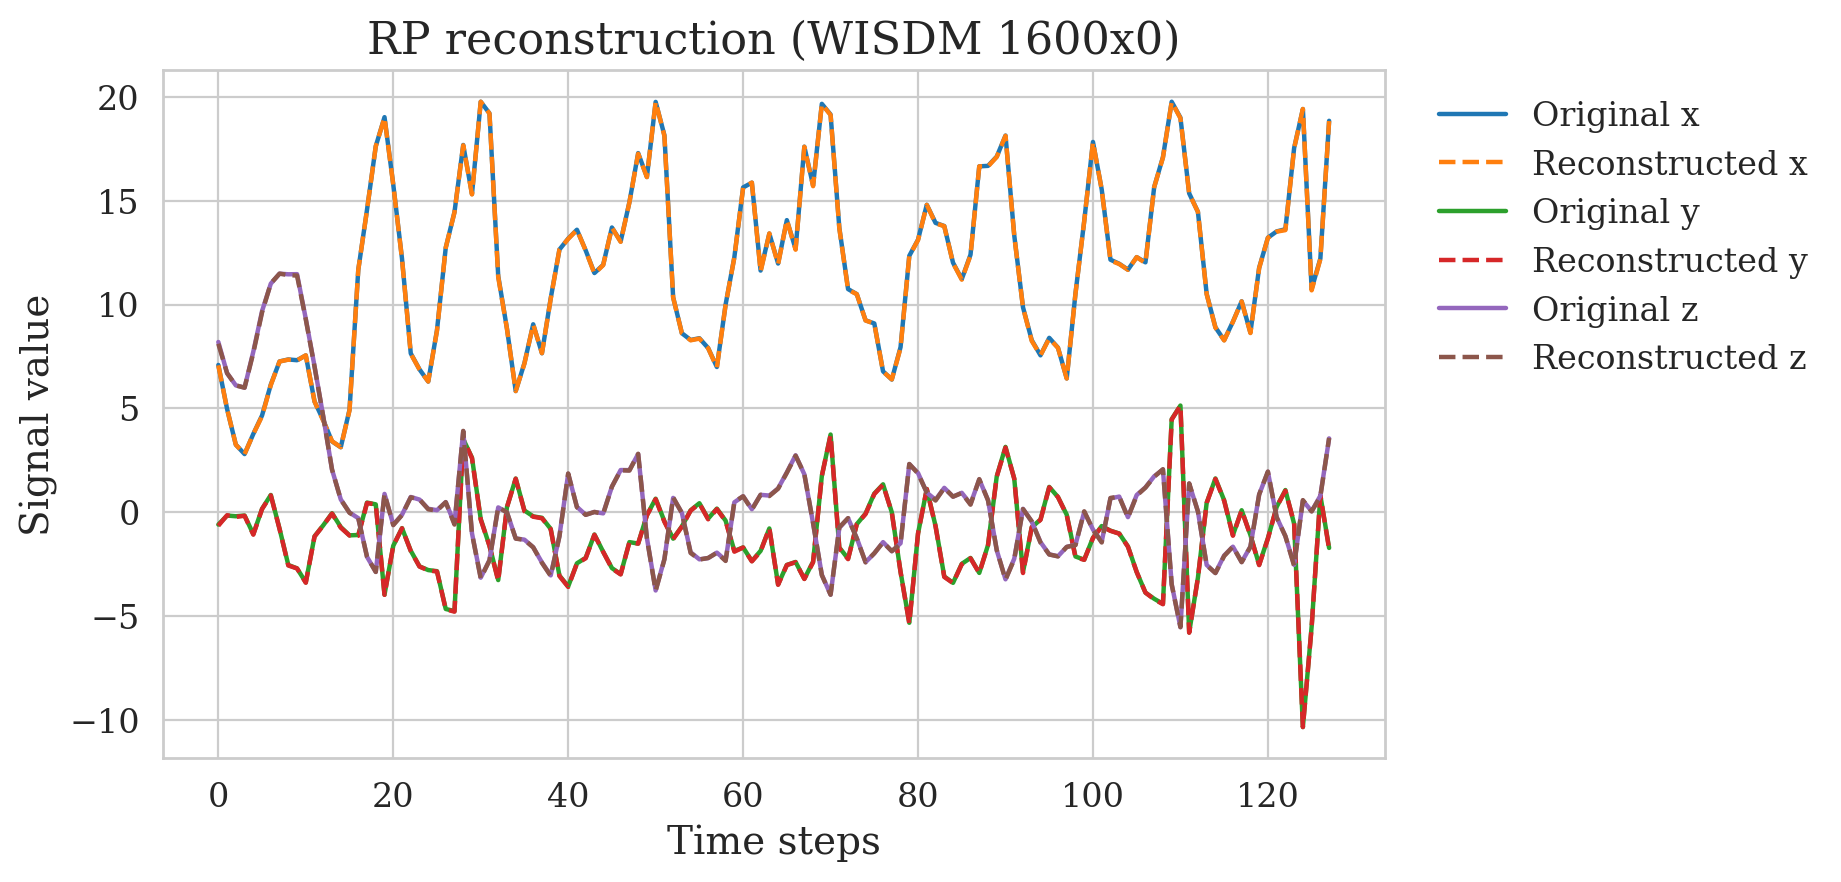
\includegraphics[width=\linewidth]{images/rp_sample_0_global.png}
\subfigtext{(a) RP}
\end{minipage}\hfill
\begin{minipage}[t]{0.48\linewidth}
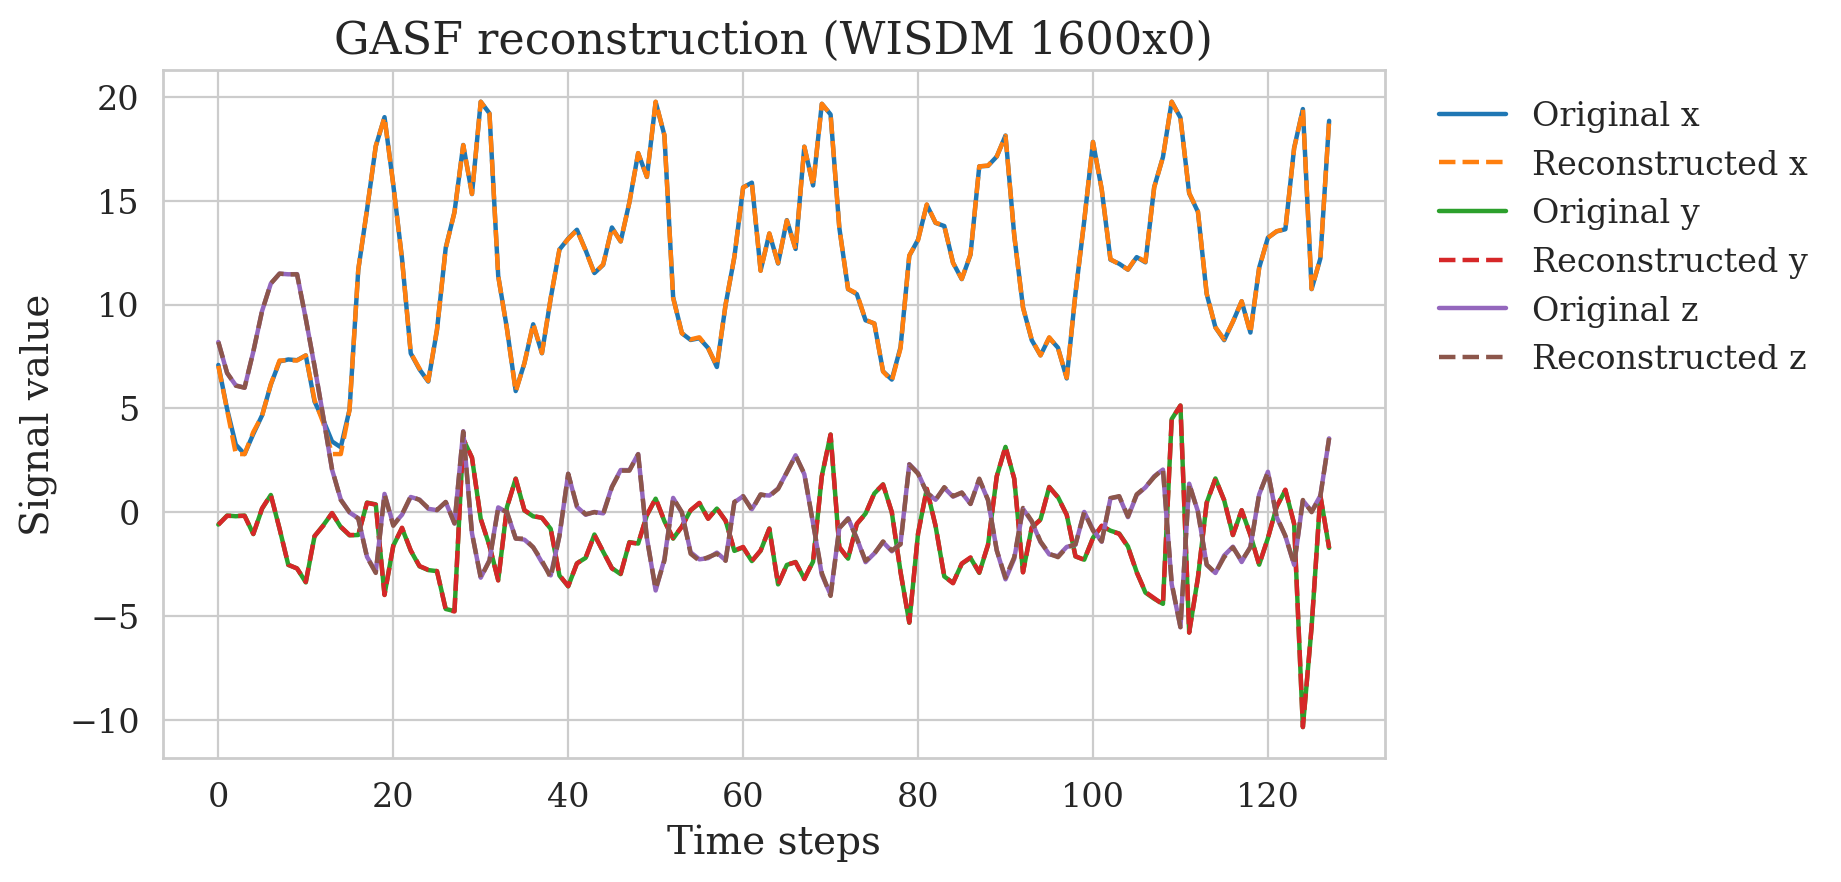
\includegraphics[width=\linewidth]{images/gaf_sample_0_global.png}
\subfigtext{(b) GASF}
\end{minipage}

\begin{minipage}[t]{0.48\linewidth}
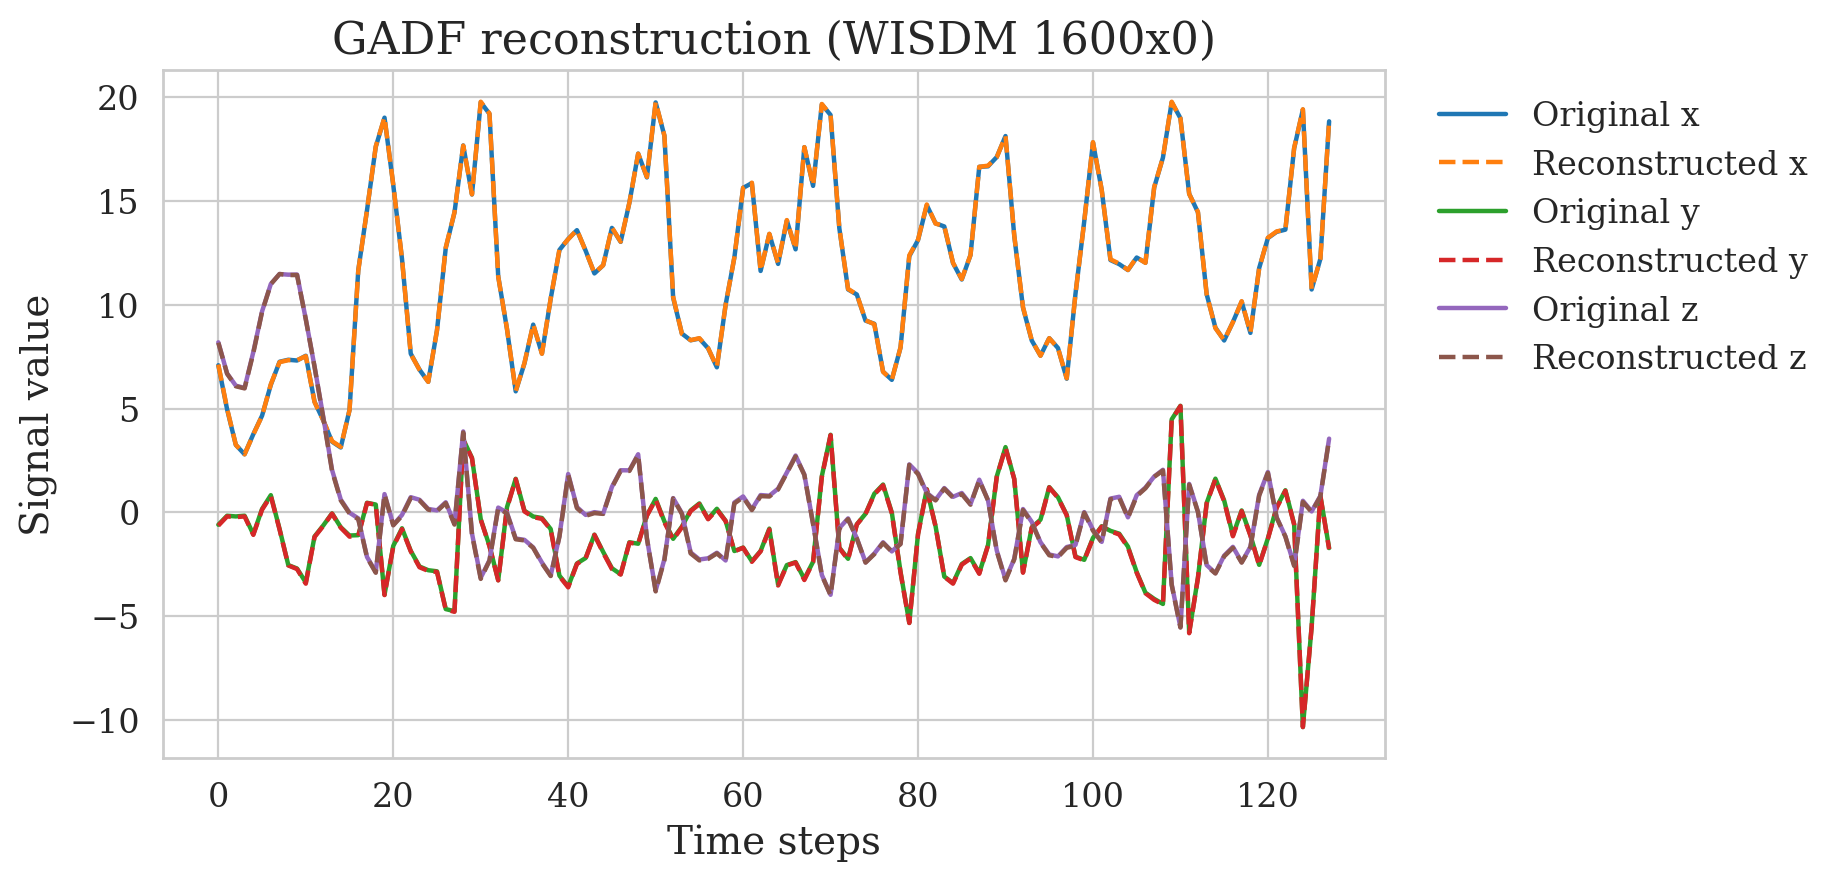
\includegraphics[width=\linewidth]{images/gadf_sample_0_global.png}
\subfigtext{(c) GADF}
\end{minipage}\hfill
\begin{minipage}[t]{0.48\linewidth}
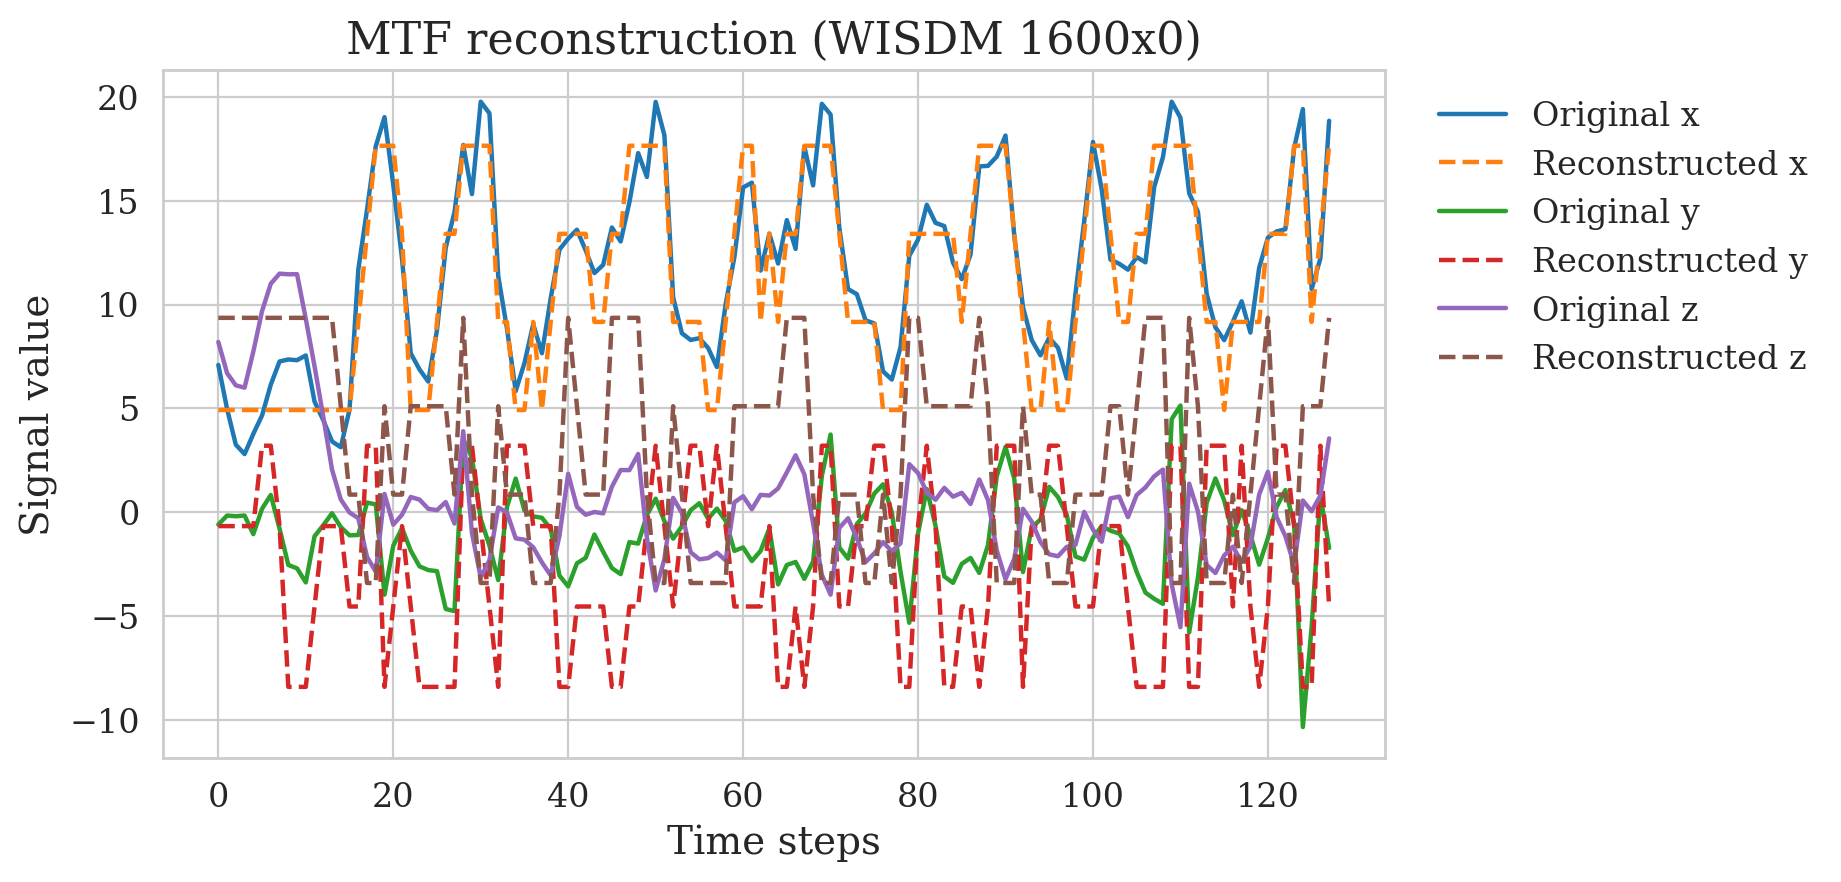
\includegraphics[width=\linewidth]{images/mtf_sample_0_global.png}
\subfigtext{(d) MTF}

\end{minipage}
\caption{Original and reconstructed triaxial signals for one WISDM walking window.}
\label{fig:qualitative_main}
\end{figure}

\subsection{Reconstruction fidelity}

Table~\ref{tab:pointwise_pooled} reports the pooled reconstruction results. Each deterministic decoder scores every one of the 8,172 windows once; the pooled values are therefore identical for the window-level and subject-out partitions. RP, GASF, and GADF operate at the 8-bit image-quantisation floor, whereas MTF is orders of magnitude less accurate pointwise. The trend lens gives the same grouping, although MTF retains a coarse cubic shape with cosine similarity 0.906.

\begin{table}[!htbp]

\centering
\caption{Pooled reconstruction fidelity over 8,172 windows. Pointwise metrics use physical units; trend cosine uses normalised cubic coefficients.}
\label{tab:pointwise_pooled}
\label{tab:normalized_metrics}
\begin{tabular}{lcccc}
\toprule
Method & MAE (mean \(\pm\) std) & MSE & Pearson & Trend cosine \\
\midrule
RP   & \(0.0148\pm0.0170\) & 0.0010 & 0.99998 & 0.99991 \\
GASF & \(0.0205\pm0.0199\) & 0.0043 & 0.99988 & 0.99975 \\
GADF & \(0.0157\pm0.0167\) & 0.0008 & 0.99999 & 1.00000 \\
MTF  & \(3.94\pm4.25\)     & 55.43  & 0.01356 & 0.90610 \\
\bottomrule
\end{tabular}
\end{table}

Paired window-level Wilcoxon tests distinguish every encoder pair after Holm correction. The practically important effect is the separation from MTF: RP, GASF, and GADF each show a large effect (\(|r|=0.866\)) against it. Differences within the near-original trio are small in absolute units despite statistical detection at \(N=8{,}172\). Repeating the test on 51 subject means preserves the MTF separation and the modest GADF-over-GASF ordering, showing that these findings are not produced solely by window-level pseudoreplication. Per-fold, per-axis, median/IQR, and cluster-bootstrap results are in the Supplementary Material.

\subsection{Downstream classification}
\label{sec:subject_out_results}

Table~\ref{tab:window_vs_subject_out} is the main classification result. Absolute accuracy decreases when whole subjects are held out, but the encoder ranking does not change: RP, GASF, and GADF track the original signal, while MTF degrades every classifier.

\begin{table}[!htbp]
\centering
\caption{Accuracy under window-level (W) and grouped subject-out (S) three-fold evaluation.}
\label{tab:window_vs_subject_out}
\resizebox{\textwidth}{!}{%
\begin{tabular}{l|cc|cc|cc|cc|cc}
\toprule
 & \multicolumn{2}{c|}{Original} & \multicolumn{2}{c|}{RP} & \multicolumn{2}{c|}{GASF} & \multicolumn{2}{c|}{GADF} & \multicolumn{2}{c}{MTF} \\
Classifier & W & S & W & S & W & S & W & S & W & S \\
\midrule
GRU  & 0.923 & 0.811 & 0.923 & 0.811 & 0.923 & 0.811 & 0.923 & 0.811 & 0.765 & 0.702 \\
KNN  & 0.642 & 0.504 & 0.642 & 0.504 & 0.642 & 0.504 & 0.643 & 0.505 & 0.559 & 0.465 \\
CNN  & 0.907 & 0.796 & 0.901 & 0.794 & 0.907 & 0.796 & 0.907 & 0.796 & 0.773 & 0.686 \\
RF   & 0.891 & 0.786 & 0.892 & 0.786 & 0.891 & 0.787 & 0.892 & 0.787 & 0.757 & 0.689 \\
SVM  & 0.801 & 0.738 & 0.802 & 0.739 & 0.801 & 0.738 & 0.801 & 0.738 & 0.697 & 0.665 \\
LSTM & 0.869 & 0.744 & 0.869 & 0.744 & 0.868 & 0.744 & 0.869 & 0.744 & 0.757 & 0.672 \\

\bottomrule
\end{tabular}}
\end{table}

Under both protocols, McNemar comparisons detect no difference between the original and RP, GASF, or GADF, or among those three (\(p_{\mathrm{Holm}}=1\) throughout), while every comparison against MTF is significant. Because failure to reject is not equivalence, we also analyse per-subject accuracy. Paired TOST confirms that RP, GASF, and GADF are equivalent to the original and to one another within the pre-specified \(\pm0.02\) margin on all six classifiers (Holm-adjusted \(p<10^{-21}\)); MTF is equivalent to none. Complete fold, class, precision, recall, F1, support, and discordant-pair tables are supplied separately.

\subsection{Decoder ablations}

\subsubsection{GADF: exactness, anchor, and pivot ensemble}
\label{sec:gadf_ablation}


The branch and anchor assumptions were checked on 1,500 WISDM windows (4,500 axis-series). The floating-point decoder is exact to numerical precision and the extreme-mean anchor has a 0\% failure rate. PNG storage introduces the observed error, which multi-pivot averaging reduces substantially.

\begin{table}[!htbp]
\centering
\caption{Core GADF ablation at \(\alpha=0.7\).}
\label{tab:gadf_npivots}
\begin{tabular}{lcc}
\toprule
Variant & MAE & Anchor failures \\
\midrule
Floating-point inverse & \(<10^{-6}\) & 0\% \\
8-bit PNG, one pivot & 0.0353 & 0\% \\
8-bit PNG, five pivots (used) & \textbf{0.0158} & 0\% \\
\bottomrule
\end{tabular}
\end{table}

The complete \(n_p\in\{1,3,5,7,9\}\) sweep, including runtime, is reported in the Supplementary Material.

\subsubsection{RP: geometry and signed orientation}
\label{sec:rp_ablation}

Table~\ref{tab:rp_ablation} separates the RP-range round-trip requirement from the two algorithmic choices. Correct inverse normalisation restores a predominantly two-dimensional Euclidean spectrum; both the full state geometry and signed orientation selection are necessary for near-lossless recovery.

\begin{table}[!htbp]
\centering
\caption{RP ablation on 100 stratified fold-0 windows. \(\mathrm{EVR}_2\) is the MDS variance in the two leading positive dimensions.}
\label{tab:rp_ablation}
\small
\begin{tabular}{lccc}
\toprule
Variant & MAE & Pearson & \(\mathrm{EVR}_2\) \\
\midrule
2-D MDS + signed orientation (proposed) & \textbf{0.010} & \textbf{1.000} & 0.947 \\
\quad signal-range decode (incorrect) & 1.047 & 0.959 & 0.218 \\
\quad without signed orientation & 2.033 & 0.794 & 0.947 \\
Prior one-dimensional graph decoder & 2.177 & 0.918 & 0.730 \\
\bottomrule

\end{tabular}
\end{table}

\subsubsection{MTF: spectral ordering}
\label{sec:mtf_ablation}

At fixed \(Q=4\), replacing cosine-pivot ordering with the Fiedler vector reduces MAE by 22\% on the 100-window ablation set, but cannot recover information lost through quantisation or the global mirror ambiguity.

\begin{table}[!htbp]
\centering
\caption{Core MTF ordering ablation at \(Q=4\).}
\label{tab:mtf_ablation}

\begin{tabular}{lcc}
\toprule
Ordering & MAE & Pearson \\
\midrule
Cosine pivot & 6.493 & \(+0.023\) \\
Fiedler vector (used) & \textbf{5.060} & \(-0.008\) \\
\bottomrule
\end{tabular}
\end{table}

The full \(Q\in\{2,4,6,8,10,16\}\) sweep selects \(Q=4\) jointly by MAE, Pearson correlation, and KNN accuracy. Variants with bin-midpoint metadata and a sign bit establish the attainable floor but are not used for the headline comparison; all extended ablations are in the Supplementary Material.

\section{Discussion}
\label{sec:discussion}

\subsection{Interpretation of the comparison}
\label{sec:disc_pointwise}
\label{sec:disc_classification}
\label{sec:disc_convergence}

The four evaluation lenses support one consistent division. RP, GASF, and GADF reconstruct the signal at the 8-bit storage floor, preserve its global trend, and remain equivalent to the raw signal for original-trained classification under both validation protocols. MTF is worse on every lens. Classification alone would not establish inversion fidelity: a coarse representation can retain class information while losing amplitude. Here the pointwise and trend metrics show that the three leading methods recover the signal itself under their stated contracts, whereas MTF preserves only a useful quantile-transition summary.

The small ordering among RP, GADF, and GASF should not obscure this result. RP has the lowest observed mean MAE, GADF the lowest MSE and highest Pearson correlation, and GASF the simplest established inverse. Their absolute differences are tiny compared with the gap to MTF, and no corresponding classification separation is detected.

\begin{table}[!htbp]
\centering
\caption{Practical interpretation of the four encodings.}
\label{tab:discussion_method_roles}
\small
\begin{tabular}{@{}L{0.09\textwidth}L{0.28\textwidth}L{0.32\textwidth}L{0.24\textwidth}@{}}
\toprule
Method & Main strength & Main constraint & Appropriate use \\
\midrule
RP & Recovers adjacent-state geometry and recurrence structure & Requires the RP-matrix range, 2-D MDS, overlap alignment, and signed orientation & Faithful inversion when recurrence geometry is analytically useful \\
GASF & Simplest closed-form diagonal inverse & Requires a fixed branch; full-range diagonal inversion loses sign & Efficient faithful baseline \\
GADF & Closed-form directional-difference recovery & Requires \(\alpha<1/\sqrt2\), fixed sign, and a reliable boundary row & Faithful difference-based inversion \\
MTF & Compact transition representation & Intrinsic quantisation and mirror ambiguity & Classification-oriented summaries \\

\bottomrule
\end{tabular}
\end{table}

Holding out complete subjects reduces absolute classifier accuracy but does not alter the encoder grouping. The subject-level TOST further turns a non-significant difference into a positive, margin-relative equivalence statement for RP, GASF, and GADF.

\subsection{Relationship between signed RP and GADF}
\label{sec:disc_structural}

Signed RP and GADF are not equivalent matrices, but both encode directional pairwise differences. For slowly varying local increments,
\[
R_{ij}\approx \sigma(i,j)\sqrt2\,|x_i-x_j|,
\qquad
G^{\mathrm D}_{ij}\approx
\frac{\bar x_j-\bar x_i}{\sqrt{1-\bar x^2}}.
\]
GADF is intrinsically antisymmetric because its sign follows from \(\sin(\phi_i-\phi_j)\); the Lu--Tong RP applies an external directional sign and need not be exactly antisymmetric. This analogy explains their visual proximity without implying a shared inverse or formal information equivalence. The full operator derivation and null-corrected regional-overlap diagnostic are provided in the Supplementary Material.

\subsection{Limitations and scope}
\label{sec:disc_scope}
\label{sec:threats}

\begin{itemize}
\item \textbf{Controlled inputs.} Every image is produced by a known encoder. Robustness to generated, noisy, occluded, or invalid images is not established, so augmentation benefit is not demonstrated.
\item \textbf{Metadata and scale.} RP needs its matrix range even for normalised reconstruction. All methods need amplitude calibration only for physical-unit output; this is not automatically available for generated images.
\item \textbf{Branch and anchor assumptions.} GASF uses a fixed branch; GADF requires \(\alpha<1/\sqrt2\), a consistent sign convention, and a detectable boundary. Near-constant or perturbed images may violate the anchor assumption.
\item \textbf{Statistical dependence.} Pooled window tests understate intra-subject dependence and combine fold-specific rules. Subject-clustered analyses reproduce the separation, but equivalence remains relative to the \(\pm0.02\) margin.
\item \textbf{External validity.} Results cover one smartwatch accelerometer dataset, five activities, 51 subjects, 20\,Hz sampling, and \(N=128\) windows.
\item \textbf{Storage precision.} The near-original tier is measured after an 8-bit PNG round trip; other formats or perturbations may change the error floor.
\end{itemize}

\subsection{Reproducibility}
\label{sec:reproducibility}

The implementation uses Python 3.10--3.11, TensorFlow 2.11--2.15, and scikit-learn. Classical MDS is deterministic; reconstructed windows retain explicit indices during parallel execution; and both fold assignments use fixed seeds. The repository includes encoders, decoders, classifiers, statistical tests, and table-generation scripts. Extended configurations and outputs are supplied in the Supplementary Material.

\section{Conclusion}
\label{sec:conclusion}

We presented three operational decoders for image-based time-series representations: a two-dimensional signed-RP inverse, a restricted-branch and boundary-anchored GADF inverse, and a Fiedler-vector MTF inverse. A GASF diagonal decoder served as the prior-art baseline. All four were evaluated on the same 8,172 WISDM windows, with the same reconstruction metrics and six original-trained classifiers under both window-level and grouped subject-out validation.

RP, GASF, and GADF form one near-original tier. Their MAEs are 0.0148, 0.0205, and 0.0157\,m/s$^2$, their temporal correlations are approximately one, and their classifier accuracies are equivalent to the raw signal within a two-percentage-point subject-level margin. They reach this result through different information: RP recovers adjacent-state geometry, GASF uses its diagonal, and GADF uses anchored angular differences. MTF remains many-to-one and is the only consistently lossy reconstruction, although its transition summary can still be useful when faithful amplitude recovery is not required.

These conclusions apply to controlled images produced by known encoders. RP requires its stored matrix range, GASF and GADF require fixed angular assumptions, and physical-unit output requires amplitude calibration. The next necessary experiment is therefore robustness to perturbed or generated images, including noise, re-quantisation, invalid anchors, and predicted rather than recorded scale.


\begin{thebibliography}{99}

\bibitem{eckmann1995recurrence}
Jean-Pierre Eckmann, S. Oliffson Kamphorst, and David Ruelle. ``Recurrence plots of dynamical systems.'' \textit{Europhysics Letters}, vol. 4, no. 9, pp. 973--977, 1987.


\bibitem{takens1981detecting}
Floris Takens. ``Detecting strange attractors in turbulence.'' In \textit{Dynamical Systems and Turbulence, Warwick 1980}, Lecture Notes in Mathematics, vol. 898, pp. 366--381, Springer, 1981.

\bibitem{marwan2007recurrence}
Norbert Marwan, M. Carmen Romano, Marco Thiel, and Jürgen Kurths. ``Recurrence plots for the analysis of complex systems.'' \textit{Physics Reports}, vol. 438, no. 5--6, pp. 237--329, 2007.

\bibitem{lu2019robust}
Jianjie Lu and Kai-Yu Tong. “Robust single accelerometer-based activity recognition using modified recurrence plot.” \textit{IEEE Sensors Journal}, vol. 19, no. 15, pp. 6317–6324, 2019.

\bibitem{THIEL2004343}
Marco Thiel, M. Carmen Romano, and Jürgen Kurths. “How much information is contained in a recurrence plot?” \textit{Physics Letters A}, vol. 330, no. 5, pp. 343–349, 2004. doi: \url{https://doi.org/10.1016/j.physleta.2004.07.050}.

\bibitem{TANIO20092031}
Masaaki Tanio, Yoshito Hirata, and Hideyuki Suzuki. “Reconstruction of driving forces through recurrence plots.” \textit{Physics Letters A}, vol. 373, no. 23, pp. 2031–2040, 2009. doi: \url{https://doi.org/10.1016/j.physleta.2009.03.069}.

\bibitem{hirata2008reproduction}
Yoshito Hirata, Shunsuke Horai, and Kazuyuki Aihara. “Reproduction of distance matrices and original time series from recurrence plots and their applications.” \textit{The European Physical Journal Special Topics}, vol. 164, no. 1, pp. 13–22, 2008.

\bibitem{cherkassky1996shortest}
Boris V. Cherkassky, Andrew V. Goldberg, and Tomasz Radzik. “Shortest paths algorithms: Theory and experimental evaluation.” \textit{Mathematical Programming}, vol. 73, no. 2, pp. 129–174, 1996.
\bibitem{wang2015encoding}
Zhiguang Wang and Tim Oates. “Imaging time-series to improve classification and imputation.” In \textit{Proceedings of the 24th International Joint Conference on Artificial Intelligence (IJCAI)}, pp. 3939--3945, 2015.

\bibitem{wang2015encoding2}
Zhiguang Wang and Tim Oates. “Encoding time series as images for visual inspection and classification using tiled convolutional neural networks.” In \textit{Workshops at the twenty-ninth AAAI Conference on Artificial Intelligence}, 2015.

\bibitem{huamin2020reconstruction}
TAO Huamin, DENG Qiuqun, and XIAO Shanzhu. “Reconstruction of time series with missing value using 2D representation-based denoising autoencoder.” \textit{Journal of Systems Engineering and Electronics}, vol. 31, no. 6, pp. 1087–1096, 2020.

\bibitem{kopec1994document}
Gary E. Kopec and Philip A. Chou. “Document image decoding using Markov source models.” \textit{IEEE Transactions on Pattern Analysis and Machine Intelligence}, vol. 16, no. 6, pp. 602–617, 1994.

\bibitem{kliewer2006iterative}
Jörg Kliewer, Norbert Goertz, and Alfred Mertins. “Iterative source-channel decoding with Markov random field source models.” \textit{IEEE Transactions on Signal Processing}, vol. 54, no. 10, pp. 3688–3701, 2006.


\bibitem{misc_wisdm_smartphone_and_smartwatch_activity_and_biometrics_dataset__507}
Gary Weiss. “WISDM Smartphone and Smartwatch Activity and Biometrics Dataset.” \textit{UCI Machine Learning Repository}, 2019. DOI: \url{https://doi.org/10.24432/C5HK59}.

\bibitem{Ding2008}
H. Ding, G. Trajcevski, P. Scheuermann, X. Wang, and E. Keogh,
``Querying and Mining of Time Series Data: Experimental Comparison of Representations and Distance Measures,''
in \emph{Proc. VLDB Endowment}, vol. 1, no. 2, pp. 1542--1552, 2008.

\bibitem{Atkins1998}
Jonathan E. Atkins, Erik G. Boman, and Bruce Hendrickson.
``A spectral algorithm for seriation and the consecutive ones problem.''
\textit{SIAM Journal on Computing}, vol. 28, no. 1, pp. 297--310, 1998. doi: \url{https://doi.org/10.1137/S0097539795285771}.


\bibitem{Botchkarev_2019}
Alexei Botchkarev. ``A New Typology Design of Performance Metrics to Measure Errors in Machine Learning Regression Algorithms.'' \textit{Interdisciplinary Journal of Information, Knowledge, and Management}, vol. 14, pp. 45--76, 2019. DOI: \url{https://doi.org/10.28945/4184}.

\bibitem{Shirkhorshidi2015}
A. S. Shirkhorshidi, S. Aghabozorgi, and T. Y. Wah, ``A comparison study on similarity and dissimilarity measures in clustering continuous data,'' \textit{PLOS ONE}, vol. 10, no. 12, pp. 1--20, 2015. doi: \url{10.1371/journal.pone.0144059}.

\bibitem{IGNATOV2018915}
Andrey Ignatov. ``Real-time human activity recognition from accelerometer data using Convolutional Neural Networks.'' \textit{Applied Soft Computing}, vol. 62, pp. 915--922, 2018. doi: \url{https://doi.org/10.1016/j.asoc.2017.09.027}.

\bibitem{Dietterich1998}
Thomas G. Dietterich. ``Approximate statistical tests for comparing supervised classification learning algorithms.'' \textit{Neural Computation}, vol. 10, no. 7, pp. 1895--1923, 1998.

\bibitem{Wilcoxon1945}
Frank Wilcoxon. ``Individual comparisons by ranking methods.'' \textit{Biometrics Bulletin}, vol. 1, no. 6, pp. 80--83, 1945.

\bibitem{Rosenthal1991}
Robert Rosenthal. \textit{Meta-Analytic Procedures for Social Research}, revised ed. Newbury Park, CA: Sage, 1991.


\bibitem{Holm1979}
Sture Holm. ``A simple sequentially rejective multiple test procedure.'' \textit{Scandinavian Journal of Statistics}, vol. 6, no. 2, pp. 65--70, 1979.
\end{thebibliography}
\end{document}
